\documentclass[10pt]{beamer}
\usetheme[left]{AAUsidebar}

% If you want to change the colors of the various elements in the theme, edit and uncomment the following lines
% Change the bar and sidebar colors:
%\setbeamercolor{AAUsidebar}{fg=red!20,bg=red}
%\setbeamercolor{sidebar}{bg=red!20}
% Change the color of the structural elements:
%\setbeamercolor{structure}{fg=red}
% Change the frame title text color:
%\setbeamercolor{frametitle}{fg=blue}
% Change the normal text color background:
%\setbeamercolor{normal text}{bg=gray!10}
% ... and you can of course change a lot more - see the beamer user manual.

\usepackage[utf8]{inputenc}
\usepackage[english]{babel}
\usepackage[T1]{fontenc}
% Or whatever. Note that the encoding and the font should match. If T1
% does not look nice, try deleting the line with the fontenc.
\usepackage{helvet}

% colored hyperlinks
\newcommand{\chref}[2]{%
  \href{#1}{{\usebeamercolor[bg]{AAUsidebar}#2}}%
}

\title[Dynamic Documents with R and knitr]% optional, use only with long paper titles
{Dynamic Documents with R and knitr}

%\subtitle{v.\ 1.4.0}  % could also be a conference name

\date{%\today
	}

\author[Leonel Muñoz Cedano] % optional, use only with lots of authors
{
  Leonel Muñoz Cedano\\
  \href{mailto:leoneling@gmail.com}{{\tt leoneling@gmail.com}}
}
% - Give the names in the same order as they appear in the paper.
% - Use the \inst{?} command only if the authors have different
%   affiliation. See the beamer manual for an example

\institute[
%  {\includegraphics[scale=0.2]{aau_segl}}\\ %insert a company, department or university logo
  Universidad Distrital Francisco José de Caldas\\
  Maestría en CIC\\
  Tendencias en IS\\
  Bogotá DC, 16 de Abril
] % optional - is placed in the bottom of the sidebar on every slide
{% is placed on the title page
  Universidad Distrital Francisco José de Caldas\\
  Maestría en Ciencias de la información y las comunicaciones\\
  Tendencias en Ingeniería de Software\\
  Bogotá DC, 16 de Abril 2016
  
  %there must be an empty line above this line - otherwise some unwanted space is added between the university and the country (I do not know why;( )
}


% specify a logo on the titlepage (you can specify additional logos an include them in 
% institute command below
\pgfdeclareimage[height=3.5cm]{titlepagelogo}{AAUgraphics/escudoudblancoynegro} % placed on the title page
%\pgfdeclareimage[height=1.5cm]{titlepagelogo2}{graphics/aau_logo_new} % placed on the title page
\titlegraphic{% is placed on the bottom of the title page
  \pgfuseimage{titlepagelogo}
%  \hspace{1cm}\pgfuseimage{titlepagelogo2}
}


\begin{document}
% the titlepage
{\aauwavesbg%
\begin{frame}[plain,noframenumbering] % the plain option removes the sidebar and header from the title page
  \titlepage
\end{frame}}
%%%%%%%%%%%%%%%%

% TOC
\begin{frame}{Agenda}{}
\tableofcontents
\end{frame}

%%%%%%%%%%%%%%%%%%%%%%%%%%%%%%%%%%%%%%%%%%%%%%%%%%%%%%%%%%%%%%%

\section{Introduction}
% motivation for creating this theme
\begin{frame}{Introduction}{}
  %The present beamer theme called the \alert{AAU Sidebar Beamer Theme} is an attempt to
  \begin{itemize}
    \item<1-> The basic idea behind dynamic documents stems from literate programming, a programming paradigm conceived by Donald Knuth (Knuth, 1984).
    \item<2->Web scripting language such as PHP (which can embed program code into HTML documents).
    \item<3->Easy manage and maintain for the author.  
    \item<4->That is why we need the literate programming paradigm. In this paradigm, an author has two tasks.
  \end{itemize}
\end{frame}
\begin{frame}{Introduction}{}
	%The present beamer theme called the \alert{AAU Sidebar Beamer Theme} is an attempt to
	Technically, literate programming involves three steps:
	\begin{itemize}
		\item<1-> Parse the source document and separate code from narratives.
		\item<1-> Execute source code and return results.
		\item<1-> Mix results from the source code with the original narratives.		
	\end{itemize}
\end{frame}
%%%%%%%%%%%%%%%%

\subsection{About the Author}
% the license
\begin{frame}{Introduction}{About the Author}
  \begin{itemize}
    \item<1->Who is \chref{http://yihui.name}{Yihui Xie}.
    \item<2->Won the 2009 John M. Chambers Statistical Software Award ( \chref{http://stat-computing.org/awards/jmc/}{ASA}).
    \item<3->Honorable Mention prize in the Applications of R in Business Contest 2012.
    \item<4->He founded the \chref{http://cos.name}{“Capital of Statistics”}.
  \end{itemize}
\end{frame}

%%%%%%%%%%%%%%%%%%%%%%%%%%%%%%%%%%%%%%%%%%%%%%%%%%%%%%%%%%%%%%%

\section{Installation}
% general installation instructions
\begin{frame}{Installation}{}  
  Installation requirements and configurations needid:
  \begin{enumerate}
    \item {\tt install \chref{https://cran.r-project.org/bin/windows/base/}{R x64} (version 3.2.3 or top)}
    \item {\tt install \chref{https://www.rstudio.com/products/rstudio/download/}{RStudio} (version 0.96.331 or top)}
    \item {\tt install packages "knitr" in R commander}
    \item {\tt install TexStudio with MiKTeX}
    \item {\tt \chref{integracion.pdf}{Integration} RStudio with TexStudio}
  \end{enumerate}
\end{frame}

\subsection{Example Knitr - code}
% the license
\begin{frame}{Installation}{Example Knitr - code}
	Example document *.Rnw in TexStudio
	
	%{\tt \textbackslash usecolortheme[<options>]\{AAUsidebar\}}\\
	{\tt \textbackslash documentclass\{article\}}\\
	{\tt \textbackslash usepackage[utf8]\{inputenc\}}\\
	{\tt \textbackslash begin\{document\}}\\
	Código de \LaTeX{} normal, puede utilizar cualquier plantilla.\\
	{\tt \textbf{<<>>=}}\\	
	{\tt \textbf{\# Crea una secuencia de números}}\\
	{\tt \textbf{X = 2:50}}\\
	{\tt \textbf{\# Muestra las medidas estadisticas basicas}}\\
	{\tt \textbf{summary(X)}}\\
	{\tt \textbf{@}}\\
	{\tt \textbackslash end\{document\}}\\
\end{frame}

\subsection{Example Knitr - result}
% the license
\begin{frame}{Installation}{Example Knitr - result}
	\vspace{1cm}
	Result of the example above
	%\vspace{-2.5cm}
	\begin{figure}[H] 
		%\centering
		\begin{flushleft}
		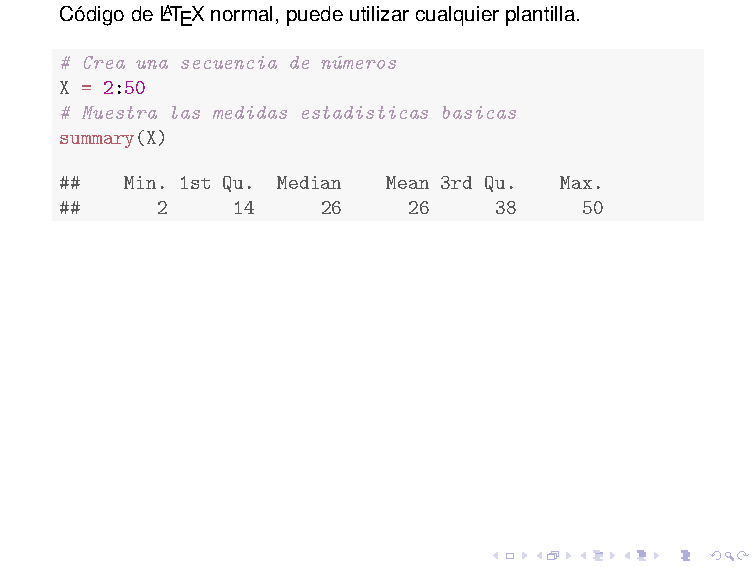
\includegraphics[width=1\textwidth]{./Rnw/document}
		\caption{Result example Knitr}
		\label{DCP}
		\end{flushleft}
	\end{figure}
\end{frame}


%%%%%%%%%%%%%%%%%%%%%%%%%%%%%%%%%%%%%%%%%%%%%%%%%%%%%%%%%%%%%%%

\section{Reproducible Research}
% general installation instructions
\begin{frame}{Reproducible Research}{}  
	Characteristics document of Reproducible research:
	\begin{itemize}
		\item<1->Results from scientific research have to be reproducible to be trustworthy.
		\item<2->Reproducible research (RR) is one possible by-product of dynamic documents.
		%\item<3->Honorable Mention prize in the Applications of R in Business Contest 2012.
		%\item<4->He founded the \chref{http://cos.name}{“Capital of Statistics”}.
	\end{itemize}
\end{frame}

\subsection{Literature}
% the Literature
\begin{frame}{Reproducible Research}{Literature}
	\begin{itemize}
		\item<1->Proposed by Jon Claerbout at Stanford University (Fomel and Claerbout, 2009).
		\item<2->Sweave (Leisch, 2002) was among the first implementations for dealing with dynamic documents in R.
		\item<3->The knitr package (Xie, 2015).
		%\item<4->He founded the \chref{http://cos.name}{“Capital of Statistics”}.
	\end{itemize}
\end{frame}

\subsection{Good and Bad Practices}
% Good and Bad Practices
\begin{frame}{Reproducible Research}{Good and Bad Practices}
	The key to keep in mind for RR is that other people should be able to
	reproduce our results. Some good practices for RR follow:
	\begin{itemize}
		\item<1->Manage all source files under the same directory and use relative
		paths whenever possible.
		\item<1->Do not change the working directory after the computing has started: function setwd().
		\item<1->Compile the documents in a clean R session.
		\item<1->Avoid the commands that require human interaction.
		\item<1->Avoid environment variables for data analysis.
		\item<1->Attach session Info and instructions on how to compile this document.
	\end{itemize}
\end{frame}

\subsection{Barriers}
% Barriers
\begin{frame}{Reproducible Research}{Barriers}
	Despite all the advantages of RR, there are some practical barriers, and here is a non-exhaustive list:
	\begin{itemize}
		\item<1->The data can be huge.
		\item<1->Confidentiality of data.
		\item<1->Software version and configuration.
		\item<1->Competition.
	\end{itemize}
\end{frame}


%%%%%%%%%%%%%%%%%%%%%%%%%%%%%%%%%%%%%%%%%%%%%%%%%%%%%%%%%%%%%%%
\section{A First Look}
% A First Look
\subsection{Setup}
% the Setup
\begin{frame}{A First Look}{Setup}
	\begin{itemize}
		\item<1->Since knitr is an R package, it can be installed from CRAN in the usual
		way in R:\\
		{\tt \textbf{install.packages("knitr", dependencies = TRUE)}}\\
		\item<1->If you have any problems with knitr, the first thing to check is its version:\\
		{\tt \textbf{packageVersion("knitr")}}\\
		{\tt \textbf{\# if not the latest version, run}}\\
		{\tt \textbf{update.packages()}}\\
		\item<1->Once we have knitr installed\\
		{\tt \textbf{library(knitr)}}\\
		{\tt \textbf{knit("your-file.Rnw")}}
	\end{itemize}
\end{frame}


\subsection{Minimal Examples}
% the Setup
\begin{frame}{A First Look}{Minimal Examples}
	{\tt \textbackslash documentclass\{article\}}\\
	{\tt \textbackslash usepackage[utf8]\{inputenc\}}\\
	{\tt \textbackslash begin\{document\}}\\
	{\tt \textbackslash title\{A Minimal Example\}}\\
	{\tt \textbackslash author\{Yihui Xie\}}\\
	{\tt \textbackslash maketitle}\\
	We examine the relationship between speed and stopping distance using a linear regression model: $Y = \beta_0 + \beta_1 x + \epsilon$.\\
	{\tt \textbf{<<model, fig.width=4, fig.height=3, fig.align='center'>>=}}\\	
	{\tt \textbf{par(mar = c(4, 4, 1, 1), mgp = c(2, 1, 0), cex = 0.8)}}\\
	{\tt \textbf{plot(cars, pch = 20, col = 'darkgray')}}\\
	{\tt \textbf{fit <- lm(dist ~ speed, data = cars)}}\\
	{\tt \textbf{abline(fit, lwd = 2)}}\\
	{\tt \textbf{@}}\\
	The slope of a simple linear regression is
	{\tt \textbackslash Sexpr\{coef(fit)[2]\}}\\
	{\tt \textbackslash end\{document\}}\\
\end{frame}
\begin{frame}{A First Look}{Minimal Examples}
	%\vspace{-2.5cm}
	\begin{figure}[H] 
		%\centering
		\begin{flushleft}
			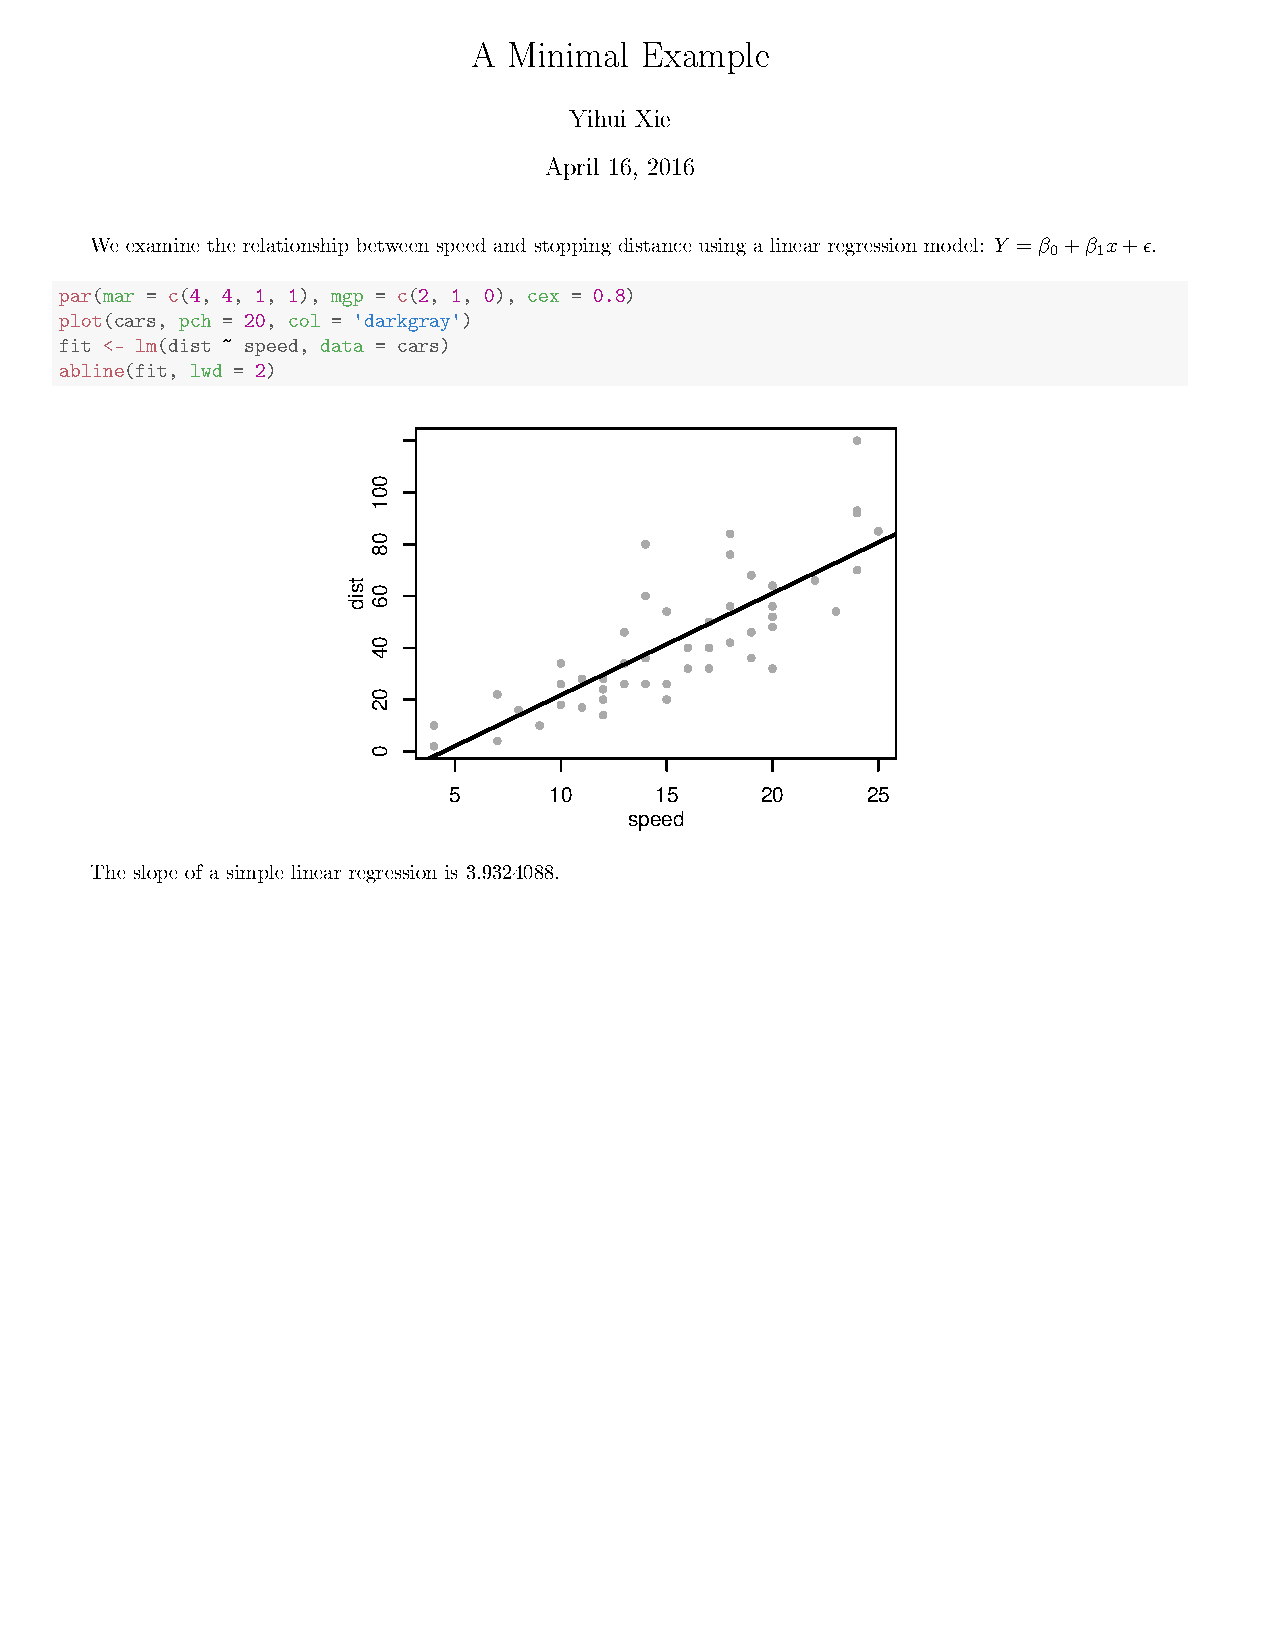
\includegraphics[width=1\textwidth]{./Rnw/minimal}
			\caption{Result example document minimal}
			\label{DCP}
		\end{flushleft}
	\end{figure}
\end{frame}

\subsection{Quick Reporting}
% the Setup
\begin{frame}{A First Look}{Quick Reporting}
	If a user only has basic knowledge of R but knows nothing about knitr, 	or one does not want to write anything other than an R script, it is also 	possible to generate a quick report from this R script using the stitch() function.\\
	\vspace{0.5cm}
	The basic idea of stitch() is that knitr provides a template of the 	source document with some default settings, so that the user only needs to feed this template with an R script (as one code chunk); then knitr will compile the template to a report. Currently it has built-in templates for LATEX, HTML, and Markdown.\\
	\vspace{0.5cm}
	The usage is like this:\\
	{\tt \textbf{library(knitr)}}\\
	{\tt \textbf{stitch("your-script.R")}}\\
	
\end{frame}

\subsection{Extracting R Code}
% the Setup
\begin{frame}{A First Look}{Extracting R Code}
	For a literate programming document, we can either compile it to a report (run the code), or extract the program code in it. They are called “weaving” and “tangling,” respectively. Apparently the function knit() is for weaving, and the corresponding tangling function is purl() in knitr. For example,\\
	\vspace{0.5cm}
	{\tt \textbf{library(knitr)}}\\
	{\tt \textbf{purl("your-file.Rnw")}}\\
	{\tt \textbf{purl("your-file.Rmd")}}\\
		
\end{frame}


%%%%%%%%%%%%%%%%%%%%%%%%%%%%%%%%%%%%%%%%%%%%%%%%%%%%%%%%%%%%%%%
\section{Feedback}
\subsection{Questions, Comments and Suggestions}
% help me iron out the bugs or give me some comment and suggestions
\begin{frame}{Feedback}{Bugs, Comments and Suggestions}
  \begin{itemize}
    \item<1-> Any Question, Comment or Suggestion.
  \end{itemize}
\end{frame}
%%%%%%%%%%%%%%%%

\subsection{Contact Information}
% contact information
\begin{frame}{Feedback}{Contact Information}
In case you have comments, suggestions or questions, please do not hesitate to contact me. You can find my contact details below.
  \begin{center}
    \insertauthor\\
  \end{center}
\end{frame}
%%%%%%%%%%%%%%%%%%%%%%%%%%%%%%%%%%%%%%%%%%%%%%%%%%%%%%%%%%%%%%%%

\section{Bibliography}
\begin{frame}{Bibliography}{}

	\begin{itemize}
		\item<1->Yihui Xie, Dynamic Documents with R and knitr, Second Edition, A Chapman and Hall Book, Taylor and Francis Group, 2015.
		\item<1->Borbón A. and Mora W., Edición de Textos Científicos LaTEX 2014, Second Edition, Escuela de Matemática, Instituto Tecnológico de Costa Rica, 2014. 
		\item<1->{\tt Pagina oficial \chref{https://cran.r-project.org/bin/windows/base/}{R x64} (version 3.2.3) https://cran.r-project.org/bin/windows/base/}.
		\item<1->Jose Nelson Pérez Castillo, Documento para Integración de RStudio con TexStudio, 2016.
	\end{itemize}
\end{frame}


%%%%%%%%%%%%%%%%%%%%%%%%%%%%%%%%%%%%%%%%%%%%%%%%%%%%%%%%%%%%%%%%


{\aauwavesbg
\begin{frame}[plain,noframenumbering]
  \finalpage{Thank you!}
\end{frame}}
%%%%%%%%%%%%%%%%

\end{document}
